%!TEX root = ../main.tex
\chapter{Testing und Qualitätssicherung}
\label{ch:testing}

Qualitätssicherung ist kein nachgelagerter Schritt, sondern ein integraler Bestandteil des Entwicklungsprozesses. Dieses Kapitel beschreibt die Teststrategie des Projekts, die eingesetzten Werkzeuge sowie die Ergebnisse der automatisierten Tests, der manuellen Verifikation, der Performance-Analyse und der Sicherheitsüberprüfung.

\section{Testkonzept und Teststrategie}
\label{sec:testkonzept}

Als konzeptioneller Rahmen dient die \textit{Testpyramide} nach Cohn \cite{contan2018}: Sie empfiehlt, den größten Anteil der Tests auf der schnellen, isolierten Unit-Ebene anzusiedeln, darüber eine mittlere Schicht aus Integrationstests zu etablieren und den Anteil aufwendiger End-to-End-Tests auf das notwendige Minimum zu beschränken. Eine invertierte Pyramide -- also eine Übergewichtung von E2E-Tests -- erzeugt lange Feedback-Zyklen, hohe Wartungskosten und fragile Testsuiten \cite{kralik2025, palli2024}. Abbildung~\ref{fig:testpyramide} zeigt die resultierende Drei-Ebenen-Struktur des Projekts.

\begin{figure}[H]
\centering
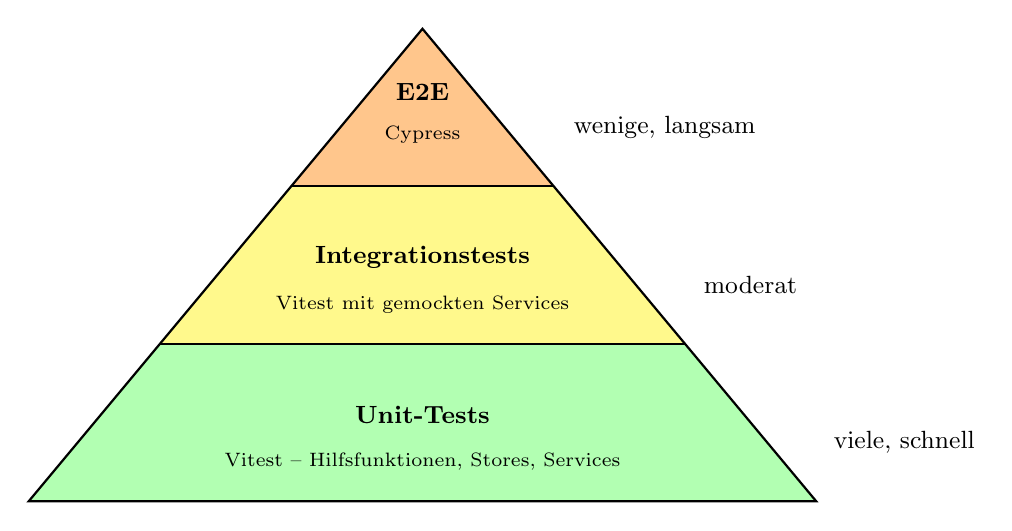
\begin{tikzpicture}[font=\small]
  % Unit Tests (bottom trapezoid) -- green
  \fill[green!30] (-5,0) -- (5,0) -- (3.33,2) -- (-3.33,2) -- cycle;
  % Integration Tests (middle trapezoid) -- yellow
  \fill[yellow!45] (-3.33,2) -- (3.33,2) -- (1.67,4) -- (-1.67,4) -- cycle;
  % E2E Tests (top triangle) -- orange
  \fill[orange!45] (-1.67,4) -- (1.67,4) -- (0,6) -- cycle;
  % Outlines
  \draw[thick] (-5,0) -- (0,6) -- (5,0) -- cycle;
  \draw[thick] (-3.33,2) -- (3.33,2);
  \draw[thick] (-1.67,4) -- (1.67,4);
  % Labels Unit Tests
  \node[align=center] at (0,1.1) {\textbf{Unit-Tests}};
  \node[align=center, font=\scriptsize] at (0,0.5) {Vitest -- Hilfsfunktionen, Stores, Services};
  % Labels Integration Tests
  \node[align=center] at (0,3.1) {\textbf{Integrationstests}};
  \node[align=center, font=\scriptsize] at (0,2.5) {Vitest mit gemockten Services};
  % Labels E2E
  \node[align=center] at (0,5.2) {\textbf{E2E}};
  \node[align=center, font=\scriptsize] at (0,4.65) {Cypress};
  % Right-side annotations
  \node[right] at (5.1,0.75) {viele, schnell};
  \node[right] at (3.45,2.75) {moderat};
  \node[right] at (1.8,4.75) {wenige, langsam};
\end{tikzpicture}
\caption{Testpyramide des Projekts nach \cite{contan2018}}
\label{fig:testpyramide}
\end{figure}

Die automatisierten Tests stützen sich auf zwei Frameworks. \textbf{Vitest} ist ein Vite-natives Test-Framework, das ECMAScript-Module nativ unterstützt und -- in Verbindung mit \texttt{happy-dom} -- Vue-Komponenten und Store-Funktionen ohne Browser-Prozess rendern und ausführen kann \cite{vitest2025}. Alle Testfälle folgen konsequent dem \textit{Arrange-Act-Assert}-Muster (AAA), das jeden Test in die drei Phasen Vorbereitung, Ausführung und Überprüfung gliedert und so die Lesbarkeit und Wartbarkeit der Suite verbessert \cite{osherove2024}. \textbf{Cypress} führt Browserinteraktionen direkt im selben JavaScript-Laufzeitkontext wie die Applikation aus, wodurch auf instabile \texttt{sleep}-Aufrufe verzichtet werden kann: Stattdessen wartet Cypress implizit auf DOM-Elemente, Netzwerkantworten und Zustandsänderungen \cite{mwaura2021, cypress2025}. Die CI-Pipeline führt beide Test-Suiten sequenziell aus -- zunächst \texttt{vitest run} für schnelles Feedback, anschließend \texttt{cypress run --e2e} im Headless-Modus -- und bricht bei einem Fehlschlag sofort ab \cite{vieira2025}.

\section{Unit-Tests}
\label{sec:unit-tests}

Die Unit-Test-Suite umfasst über 200 Testfälle, die in vier Dateien unter \texttt{tests/unit/} organisiert sind und drei Schichten der Anwendung abdecken. Das Testprinzip folgt dabei der Idee der maximalen Isolation: Jede Einheit wird ausschließlich mit ihren eigenen Eingaben und Ausgaben geprüft; externe Abhängigkeiten werden vollständig durch Mocks ersetzt \cite{osherove2024}.

\paragraph{Hilfsfunktionen.} Die Datei \texttt{utils.test.js} prüft alle acht reinen Funktionen aus \texttt{src/utils/index.js} vollständig ohne Mocking, da diese ausschließlich auf Eingabeparametern operieren. Getestet werden unter anderem \texttt{formatPrice} (Euroformatierung mit Tausendertrennzeichen), \texttt{isValidEmail} (Erkennung gültiger und ungültiger E-Mail-Adressen), \texttt{calculateDiscountPrice} (korrekte Rabattberechnung inklusive Grenzfällen) sowie \texttt{getStockStatus} und \texttt{getStockClass} (Ableitung von Lagerstatustext und CSS-Klasse aus numerischen Bestandswerten). Jede Funktion erhält Testfälle für Normalwerte, Grenzwerte (z.\,B. Preis\,=\,0) und Fehlereingaben.

\paragraph{Store-Logik.} Die Dateien \texttt{cartStore.test.js} und \texttt{wishlistStore.test.js} testen die reaktiven Zustandsfunktionen \texttt{updateCartCount}, \texttt{updateCartItems} bzw. ihre Äquivalente im Wunschlisten-Store. Da die Store-Funktionen intern auf die Serviceschicht zugreifen, wird diese über \texttt{vi.mock()} durch kontrollierbare Stubs ersetzt. Die Tests verifizieren, dass nach einem Serviceaufruf die exportierten Composables (\texttt{useCartItemCount}, \texttt{useCartItems}) den korrekten reaktiven Wert liefern -- unabhängig davon, ob Firebase erreichbar ist.

\paragraph{Suchdienste.} Die Service-Tests unter \texttt{tests/unit/services/} isolieren die Funktionen \texttt{searchProducts} und \texttt{getSearchSuggestions} mit einem kontrollierten Mock-Produktportfolio, das verschiedene Kategorien, Lagerzustände und Preisbereiche abbildet. So wird sichergestellt, dass Filterlogik, Scoring und Trefferrangfolge korrekt implementiert sind.

\section{End-to-End-Tests}
\label{sec:e2e-tests}

Die E2E-Tests operieren auf der vollständig gerenderten Anwendung im Browser und prüfen Nutzungsflüsse so, wie ein realer Nutzer sie erlebt -- von der Seitennavigation über Formulareingaben bis hin zu asynchronen Firestore-Operationen \cite{mwaura2021, palli2024}. Die acht Spec-Dateien unter \texttt{tests/e2e/} decken die gesamte Breite der Anwendungsfunktionalität ab: Authentifizierung, Warenkorb, Checkout, Navigation, Angebote, Produktbrowsing, Suche und Wunschliste.

Wiederkehrende Operationen wie das Einloggen (\texttt{cy.login()}), das Leeren des Warenkorbs (\texttt{cy.clearCart()}) oder das Akzeptieren des Cookie-Banners (\texttt{cy.acceptCookies()}) sind als Custom Commands in \texttt{tests/support/commands.js} gekapselt. Dieses Muster reduziert Codeduplizierung und erleichtert die Anpassung bei Änderungen der UI \cite{cypress2025, vieira2025}. Jede Spec-Datei stellt per \texttt{beforeEach}-Hook einen definierten Ausgangszustand her und prüft neben dem Erfolgsfall (Happy Path) systematisch auch Fehlerpfade: So muss der Checkout-Button bei leerem Warenkorb unsichtbar bleiben, der Aufruf einer geschützten Route ohne aktive Sitzung auf \texttt{/login} umleiten und eine ungültige Produkt-URL die 404-Seite anzeigen. Der Checkout-Flow selbst wird mehrstufig verifiziert -- von der Produktdetailseite über den Warenkorb bis zum Bestellformular mit Adress- und Zahlungsfeldern. Für Mobile-Viewpoints kommt zusätzlich \texttt{cy.viewport('iphone-x')} zum Einsatz, um sicherzustellen, dass kritische UI-Elemente auch auf kleinen Bildschirmen korrekt dargestellt werden.

\section{Manuelle Tests, Cross-Browser und Responsive Design}
\label{sec:manuelle-tests}

Nicht alle Qualitätsaspekte lassen sich vollständig automatisieren. Ergänzend zu den automatisierten Suiten wurden daher manuelle Funktionstests durchgeführt, die insbesondere den Google-OAuth-Fluss, das Admin-Dashboard, die Cookie-Einstellungen sowie die visuelle Konsistenz der Benutzeroberfläche abdecken. Diese Tests erfolgten iterativ während der Implementierungsphase und wurden bei UI-Änderungen wiederholt.

Cross-Browser-Inkompatibilitäten entstehen durch unterschiedliche Rendering-Engines und können -- trotz standardkonformem Code -- zu abweichenden Layouts oder Funktionsstörungen führen \cite{watanabe2023}. Alle wesentlichen Benutzerflüsse wurden daher manuell in Google Chrome (Blink-Engine), Mozilla Firefox (Gecko) und Safari (WebKit) verifiziert. Herstellerspezifische CSS-Präfixe ergänzt der Vite-interne PostCSS-Prozessor automatisch, sodass manuelle Vendor-Prefix-Pflege entfällt. Das Mobile-First-Layout mit definierten Breakpoints bei 768\,px (Tablet) und 1024\,px (Desktop) zeigte in allen getesteten Browsern und Gerätegrößen ein konsistentes Erscheinungsbild.

\section{Performance-Analyse}
\label{sec:performance}

Die Performance-Analyse wurde mit Google Lighthouse auf dem produktiven Firebase-Hosting-Endpunkt nach einem vollständigen Produktionsbuild (\texttt{vite build}) durchgeführt. Lighthouse bewertet Webseiten anhand der \textit{Core Web Vitals} -- Largest Contentful Paint (LCP, Zielwert $\leq\,2{,}5$\,s), Interaction to Next Paint (INP, $\leq\,200$\,ms) und Cumulative Layout Shift (CLS, $\leq\,0{,}1$) -- sowie weiterer Metriken wie Time to First Byte und Total Blocking Time \cite{jainweb2023, dobbala2022}.

Die Startseite erzielte einen Performance-Score von 91, die Produktdetailseite von 88; beide Seiten erreichten 100 Punkte in der Kategorie Best Practices. Die hohen Werte sind auf ein Zusammenspiel mehrerer Optimierungsmaßnahmen zurückzuführen: Vites Tree-Shaking und automatisches Code-Splitting reduzieren die initiale Bundle-Größe erheblich, indem unused Code zur Build-Zeit entfernt und seitenspezifische Chunks erst bei Bedarf geladen werden. Die CDN-basierte Auslieferung über Firebase Hosting mit HTTP/2-Multiplexing und Gzip-Kompression minimiert die Übertragungslatenz. Produktbilder werden mit dem nativen \texttt{loading="lazy"}-Attribut nachgeladen, sodass beim initialen Seitenaufruf nur die sichtbaren Bilder transferiert werden. Der minimal niedrigere Performance-Score der Produktdetailseite ist systembedingt auf den synchronen Firestore-Datenabruf zurückzuführen: Der primäre Seiteninhalt kann erst nach der Datenbankabfrage gerendert werden, was den LCP-Wert geringfügig erhöht.

\section{Sicherheitsüberprüfung}
\label{sec:sicherheit-test}

Unzureichende Authentifizierung und fehlerhafte Zugriffskontrolle gehören laut OWASP Top 10 zu den kritischsten Sicherheitsrisiken für Webanwendungen \cite{wen2023, fredj2020}. Die Sicherheitsarchitektur des Webshops begegnet diesen Risiken auf zwei Ebenen: dem clientseitigen Routing-Schutz und den serverseitigen Firestore Security Rules.

Firebase Authentication übernimmt das vollständige Credential-Management: Passwörter werden ausschließlich serverseitig gehasht und gesalzen gespeichert; clientseitig sind zu keinem Zeitpunkt Klartextpasswörter oder Hashes zugänglich. JWTs werden von Firebase automatisch ausgestellt, kryptografisch signiert und nach Ablauf der Gültigkeit (Standard: 1\,h) transparent erneuert \cite{bucko2023, firebaseAuth2025}. Die clientseitige Zugriffskontrolle ist über einen globalen Vue-Router-Guard realisiert, der die Metafelder \texttt{requiresAuth} und \texttt{requiresAdmin} jeder Routendefinition auswertet: Ein direkter Aufruf von \texttt{/profile} oder einer Admin-Route ohne aktive Sitzung löst eine sofortige Weiterleitung auf \texttt{/login} aus. Die Überprüfung wurde im Rahmen der E2E-Tests automatisiert verifiziert.

Da Firebase-Projekte ohne serverseitige Applikationsschicht direkt aus dem Browser auf Firestore zugreifen, bilden die \textit{Security Rules} die einzige Zugriffskontrollschranke zwischen Client und Datenbank -- fehlerhafte Rules können dazu führen, dass beliebige Nutzer fremde Daten lesen oder überschreiben \cite{milojkovic2024}. Die Rules des Projekts definieren vier wiederverwendbare Hilfsfunktionen:

\begin{lstlisting}[language={}, morekeywords={function,return,allow,match,if,true,false,write,read,get,create,update,delete,request,resource,auth,data,databases,documents}, caption=Hilfsfunktionen der Firestore Security Rules (firestore.rules)]
function isAuthenticated() {
  return request.auth != null;
}
function isOwner(userId) {
  return isAuthenticated() && request.auth.uid == userId;
}
function isAdmin() {
  return isAuthenticated() &&
    get(/databases/$(database)/documents/users/$(request.auth.uid))
      .data.role == 'admin';
}
function noRoleEscalation() {
  return !('role' in request.resource.data) ||
    request.resource.data.role == resource.data.role;
}
\end{lstlisting}

Die Funktion \texttt{noRoleEscalation()} verhindert, dass ein angemeldeter Nutzer beim Update des eigenen Dokuments das \texttt{role}-Feld von \texttt{'user'} auf \texttt{'admin'} eskalieren kann -- ein klassisches Privilege-Escalation-Szenario, das zur OWASP-Kategorie \textit{Broken Access Control} zählt \cite{wen2023}. Öffentlich lesbare Kollektionen wie \texttt{products}, \texttt{categories} und \texttt{offers} erlauben Schreibzugriff ausschließlich für Admins. Die \texttt{users}-Kollektion schützt Nutzer vor gegenseitigen Zugriffen: Lesen und Schreiben sind strikt auf das eigene Dokument beschränkt. Besonders sorgfältig abgesichert ist die \texttt{orders}-Kollektion: Neue Bestellungen müssen zwingend den Status \texttt{'pending'} tragen, sodass ein Angreifer keine Bestellung mit dem Status \texttt{'shipped'} oder \texttt{'paid'} direkt einschleusen kann. Statusübergänge sind ausschließlich dem Admin-Dashboard und den Cloud Functions via Admin SDK vorbehalten. Die Kollektion \texttt{newsletterLogs} ist für Clientzugriffe vollständig gesperrt.

Die Korrektheit der Rules wurde manuell im Firebase Emulator verifiziert: Zugriffe nicht authentifizierter Nutzer auf \texttt{/users}-Dokumente wurden mit \texttt{PERMISSION\_DENIED} abgelehnt, und der Versuch einer Rollenerhöhung durch einen regulären Nutzer wurde korrekt blockiert.
